% Options for packages loaded elsewhere
\PassOptionsToPackage{unicode}{hyperref}
\PassOptionsToPackage{hyphens}{url}
\PassOptionsToPackage{dvipsnames,svgnames,x11names}{xcolor}
%
\documentclass[
]{article}
\usepackage{amsmath,amssymb}
\usepackage{lmodern}
\usepackage{iftex}
\ifPDFTeX
  \usepackage[T1]{fontenc}
  \usepackage[utf8]{inputenc}
  \usepackage{textcomp} % provide euro and other symbols
\else % if luatex or xetex
  \usepackage{unicode-math}
  \defaultfontfeatures{Scale=MatchLowercase}
  \defaultfontfeatures[\rmfamily]{Ligatures=TeX,Scale=1}
\fi
% Use upquote if available, for straight quotes in verbatim environments
\IfFileExists{upquote.sty}{\usepackage{upquote}}{}
\IfFileExists{microtype.sty}{% use microtype if available
  \usepackage[]{microtype}
  \UseMicrotypeSet[protrusion]{basicmath} % disable protrusion for tt fonts
}{}
\makeatletter
\@ifundefined{KOMAClassName}{% if non-KOMA class
  \IfFileExists{parskip.sty}{%
    \usepackage{parskip}
  }{% else
    \setlength{\parindent}{0pt}
    \setlength{\parskip}{6pt plus 2pt minus 1pt}}
}{% if KOMA class
  \KOMAoptions{parskip=half}}
\makeatother
\usepackage{xcolor}
\usepackage[margin=1in]{geometry}
\usepackage{longtable,booktabs,array}
\usepackage{calc} % for calculating minipage widths
% Correct order of tables after \paragraph or \subparagraph
\usepackage{etoolbox}
\makeatletter
\patchcmd\longtable{\par}{\if@noskipsec\mbox{}\fi\par}{}{}
\makeatother
% Allow footnotes in longtable head/foot
\IfFileExists{footnotehyper.sty}{\usepackage{footnotehyper}}{\usepackage{footnote}}
\makesavenoteenv{longtable}
\usepackage{graphicx}
\makeatletter
\def\maxwidth{\ifdim\Gin@nat@width>\linewidth\linewidth\else\Gin@nat@width\fi}
\def\maxheight{\ifdim\Gin@nat@height>\textheight\textheight\else\Gin@nat@height\fi}
\makeatother
% Scale images if necessary, so that they will not overflow the page
% margins by default, and it is still possible to overwrite the defaults
% using explicit options in \includegraphics[width, height, ...]{}
\setkeys{Gin}{width=\maxwidth,height=\maxheight,keepaspectratio}
% Set default figure placement to htbp
\makeatletter
\def\fps@figure{htbp}
\makeatother
\setlength{\emergencystretch}{3em} % prevent overfull lines
\providecommand{\tightlist}{%
  \setlength{\itemsep}{0pt}\setlength{\parskip}{0pt}}
\setcounter{secnumdepth}{5}
\ifLuaTeX
  \usepackage{selnolig}  % disable illegal ligatures
\fi
\usepackage[]{natbib}
\bibliographystyle{biochem}
\IfFileExists{bookmark.sty}{\usepackage{bookmark}}{\usepackage{hyperref}}
\IfFileExists{xurl.sty}{\usepackage{xurl}}{} % add URL line breaks if available
\urlstyle{same} % disable monospaced font for URLs
\hypersetup{
  pdftitle={Supplementary Figures: Quality control for the target decoy approach for peptide identification},
  pdfauthor={Elke Debrie\^{}1 Milan Malfait\^{}1 Ralf Gabriels\^{}\{2,3\} Arthur Declerq\^{}\{2,3\} Adriaan Sticker\^{}\{2,3\} Lennart Martens\^{}\{2,3\} Lieven Clement\^{}\{1,4\}},
  colorlinks=true,
  linkcolor={blue},
  filecolor={Maroon},
  citecolor={blue},
  urlcolor={blue},
  pdfcreator={LaTeX via pandoc}}

\title{Supplementary Figures: Quality control for the target decoy approach for peptide identification}
\author{Elke Debrie\(^1\) Milan Malfait\(^1\) Ralf Gabriels\(^{2,3}\) Arthur Declerq\(^{2,3}\) Adriaan Sticker\(^{2,3}\) Lennart Martens\(^{2,3}\) Lieven Clement\(^{1,4}\)}
\date{\(^1\) Department of Applied Mathematics, Computer Science and Statistics, Ghent University, Ghent, Belgium \newline \(^2\) VIB-UGent Center for Medical Biotechnology, VIB, Zwijnaarde, Belgium \newline \(^3\) Department of Biomolecular Medicine, Ghent University, Ghent, Belgium \newline \(^4\) Corresponding Author\(:\) \href{mailto:lieven.clement@ugent.be}{\nolinkurl{lieven.clement@ugent.be}}}

\begin{document}
\maketitle

\setcitestyle{super,open={[},close={]}}
\def\citenumfont{}



\begin{figure}
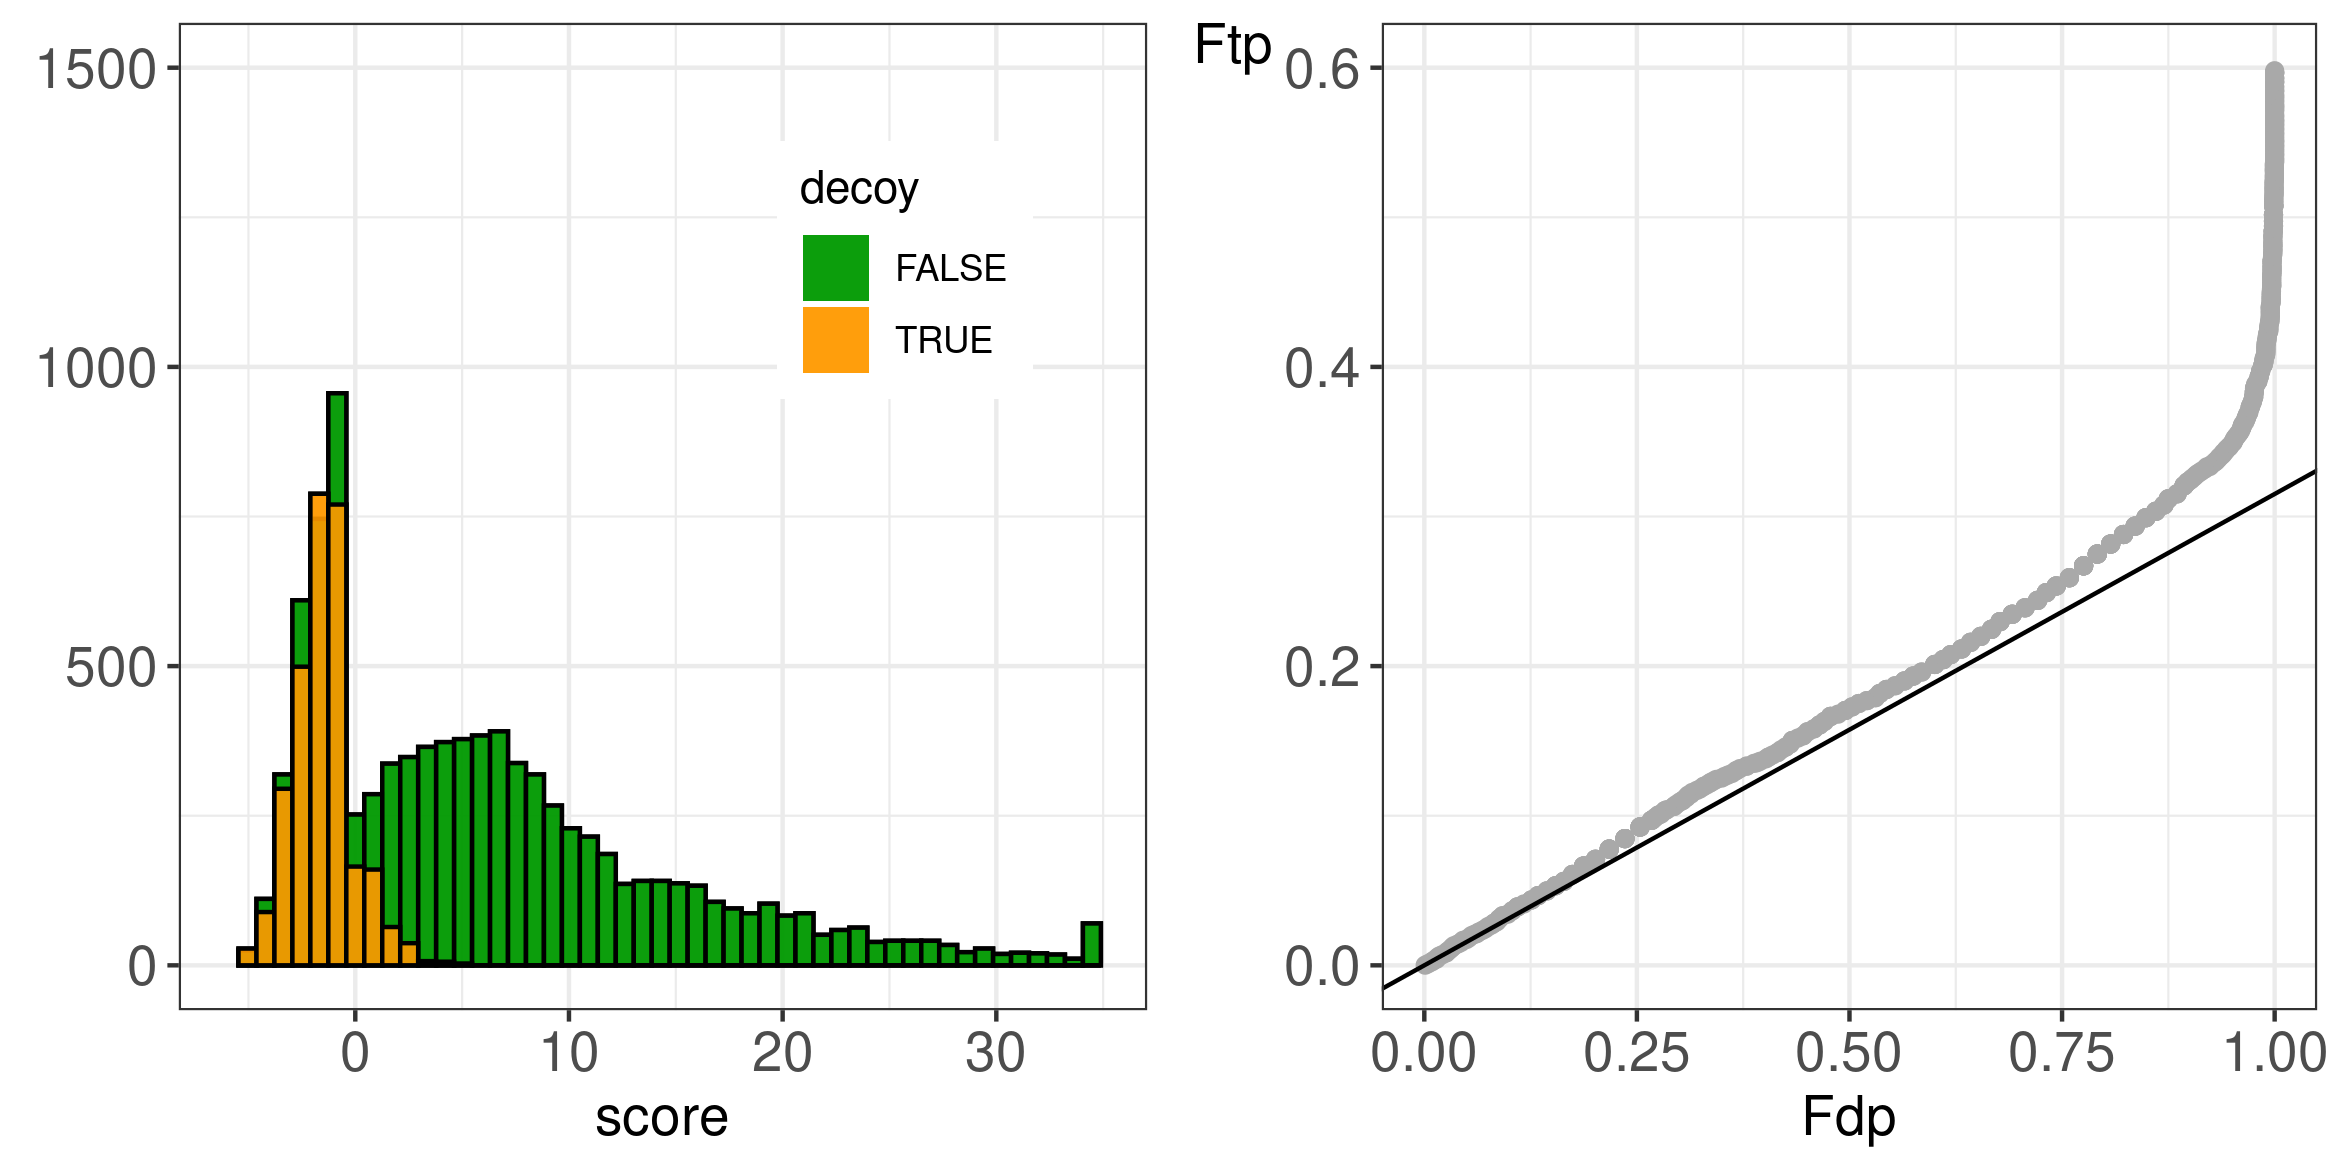
\includegraphics[width=0.99\linewidth]{./figs/figTandemNoRefineSwissHistPP} \caption{Histogram and PP-plot for a concatenated search on a \emph{Pyrococcus} run against a database of canonical \emph{P. furiosus} sequences from Swiss-Prot using X!Tandem without refinement. Both the histogram and the P-P plot show no violation of the TDA assumptions.}\label{fig:sFig1}
\end{figure}



\begin{figure}
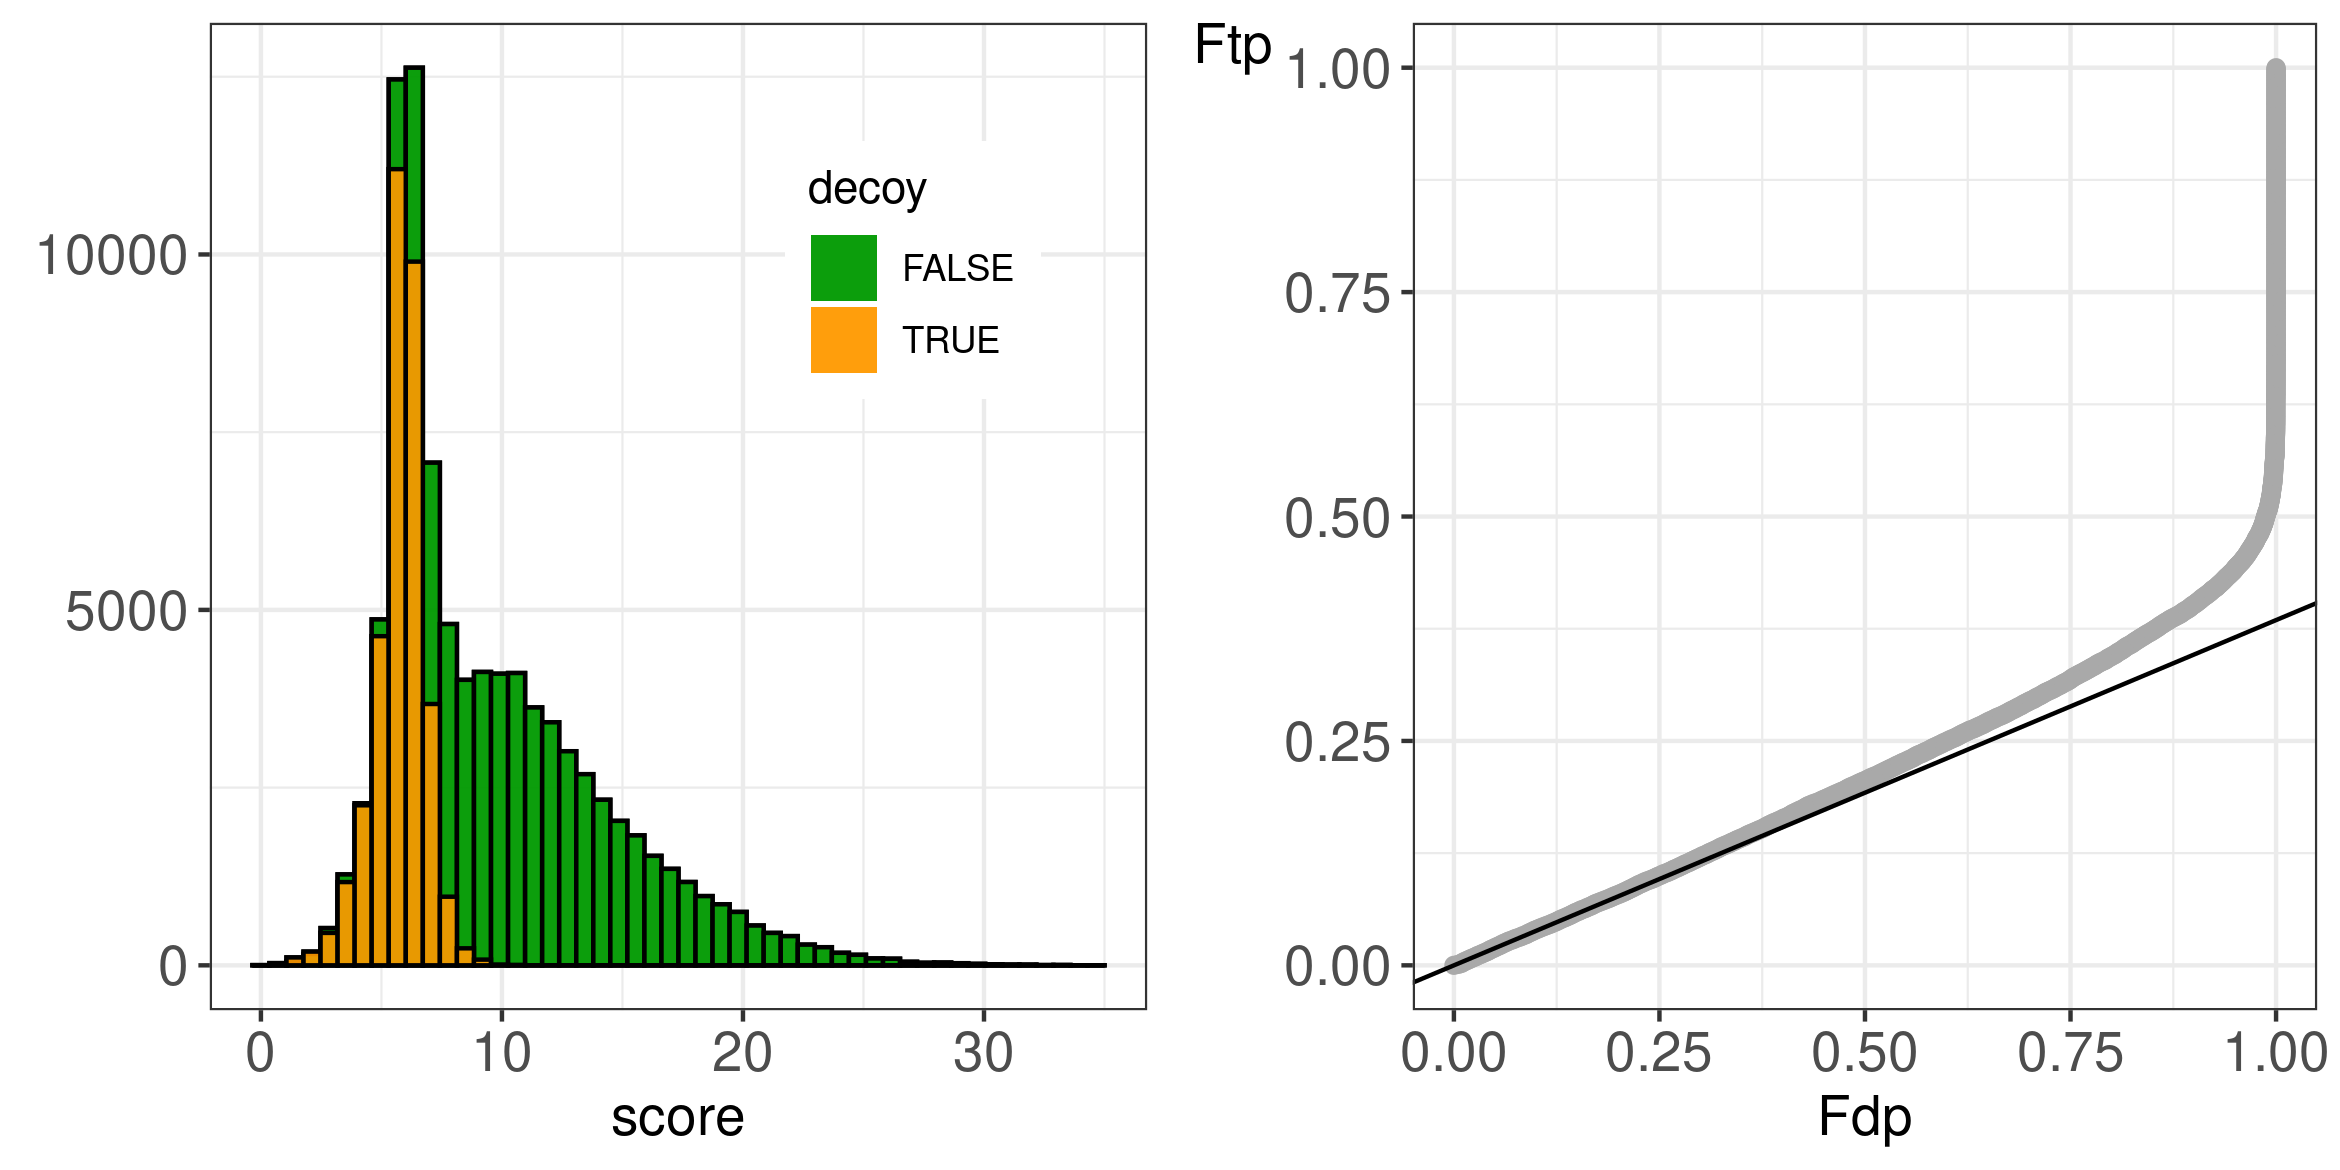
\includegraphics[width=0.99\linewidth]{./figs/figHumanMsgfPlus} \caption{Histogram and PP-plot for a concatenated search on a \emph{H. sapiens} run against a database of \emph{H. Sapiens} sequences from UniProt using MS-GF+. Both the histogram and the P-P plot show no violation of the TDA assumptions.}\label{fig:sFig2}
\end{figure}



\begin{figure}
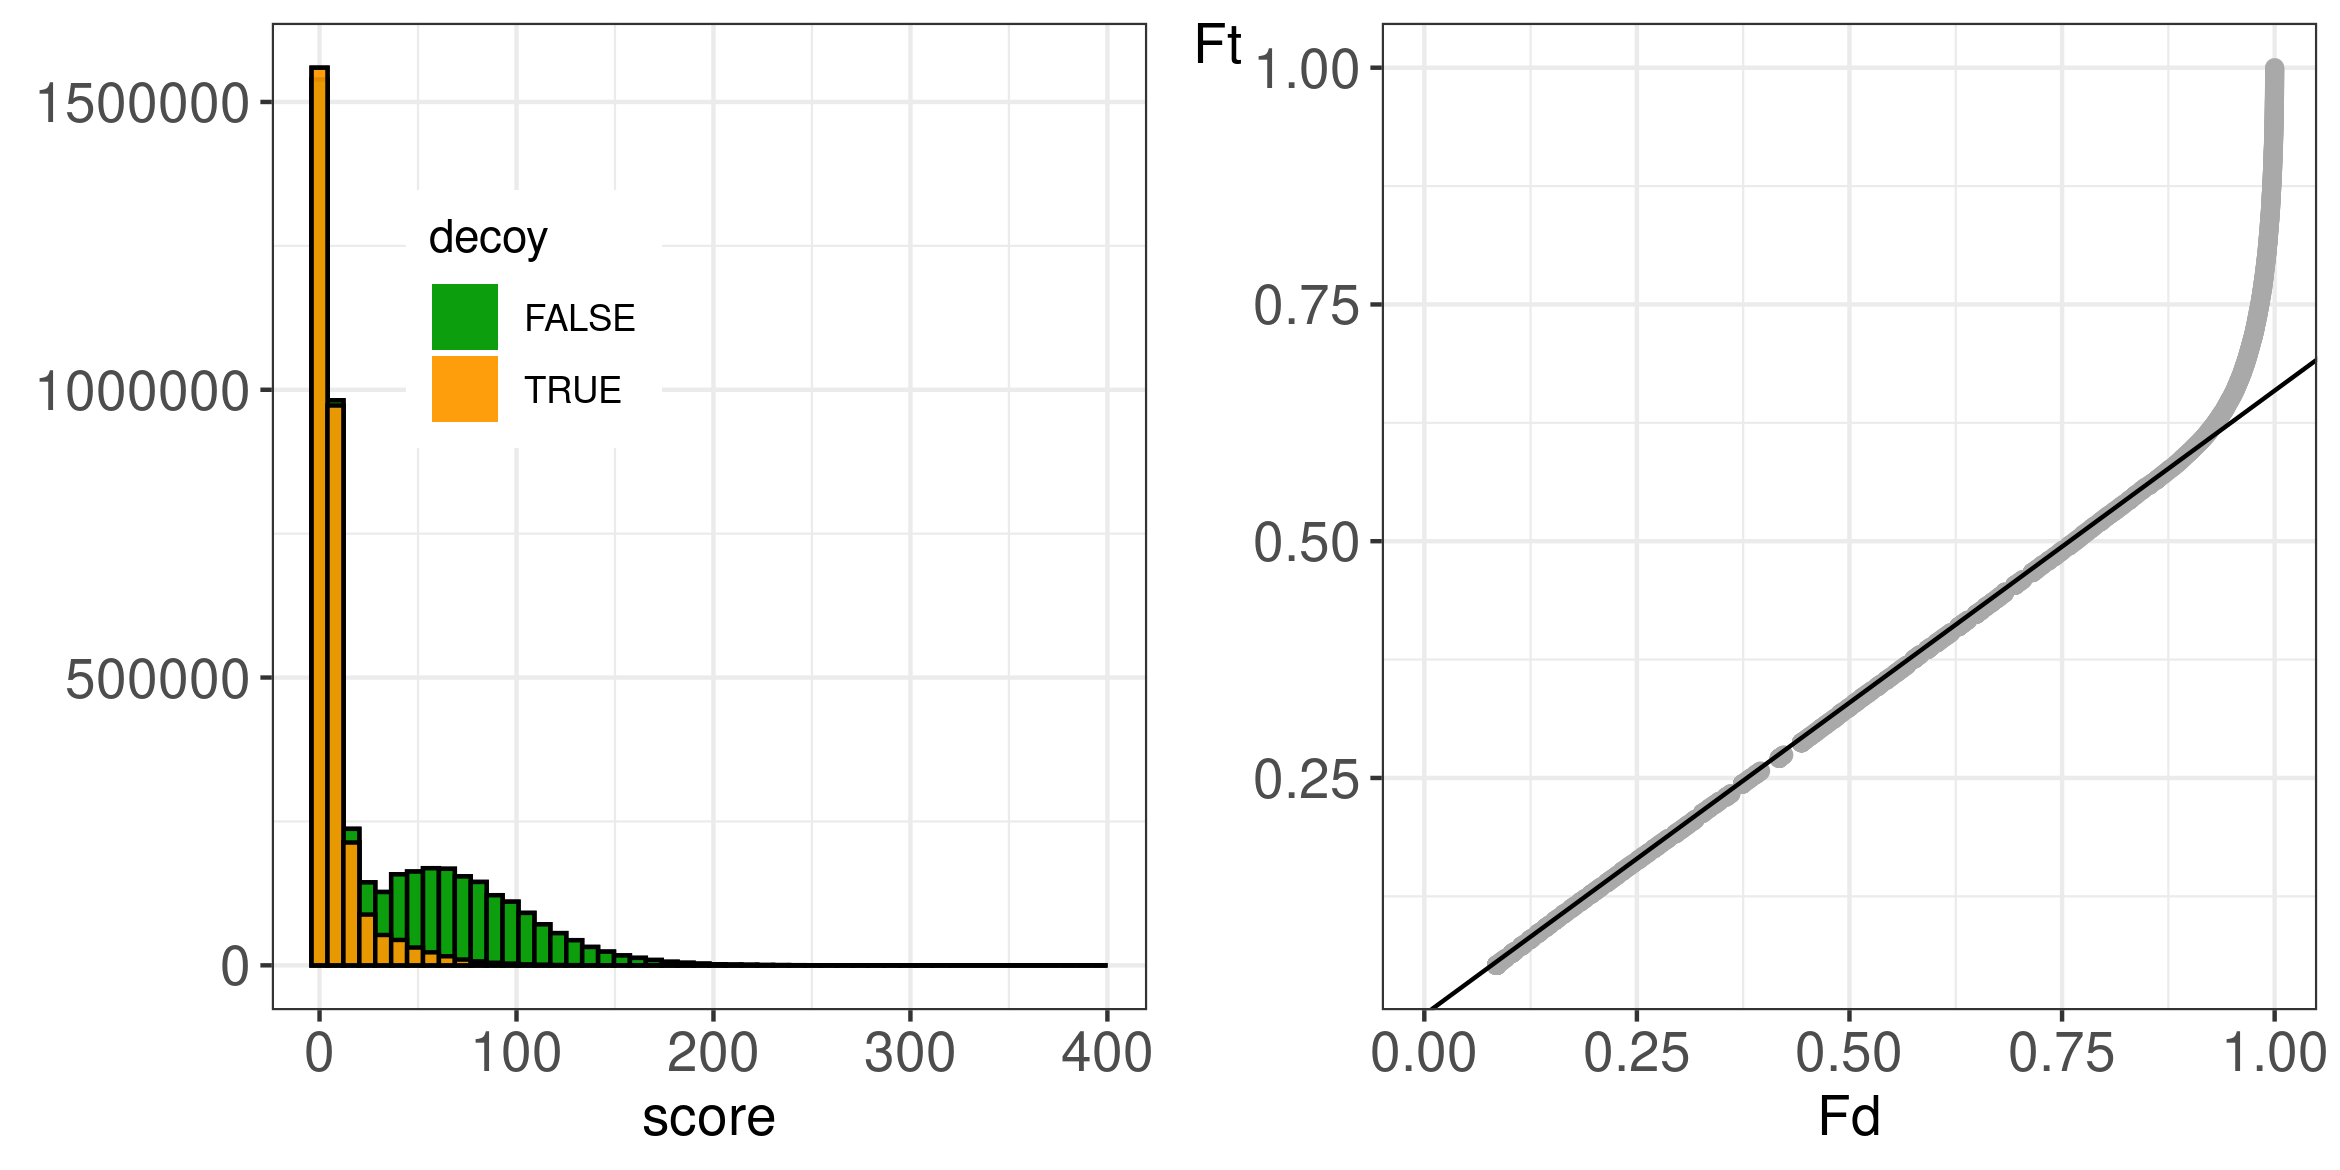
\includegraphics[width=0.99\linewidth]{./figs/figPeptidomics} \caption{Histogram and PP-plot for a concatenated search on an immunopeptidomics run using Andromeda. Both the histogram and the P-P plot show no violation of the TDA assumptions.}\label{fig:sFig3}
\end{figure}



\begin{figure}
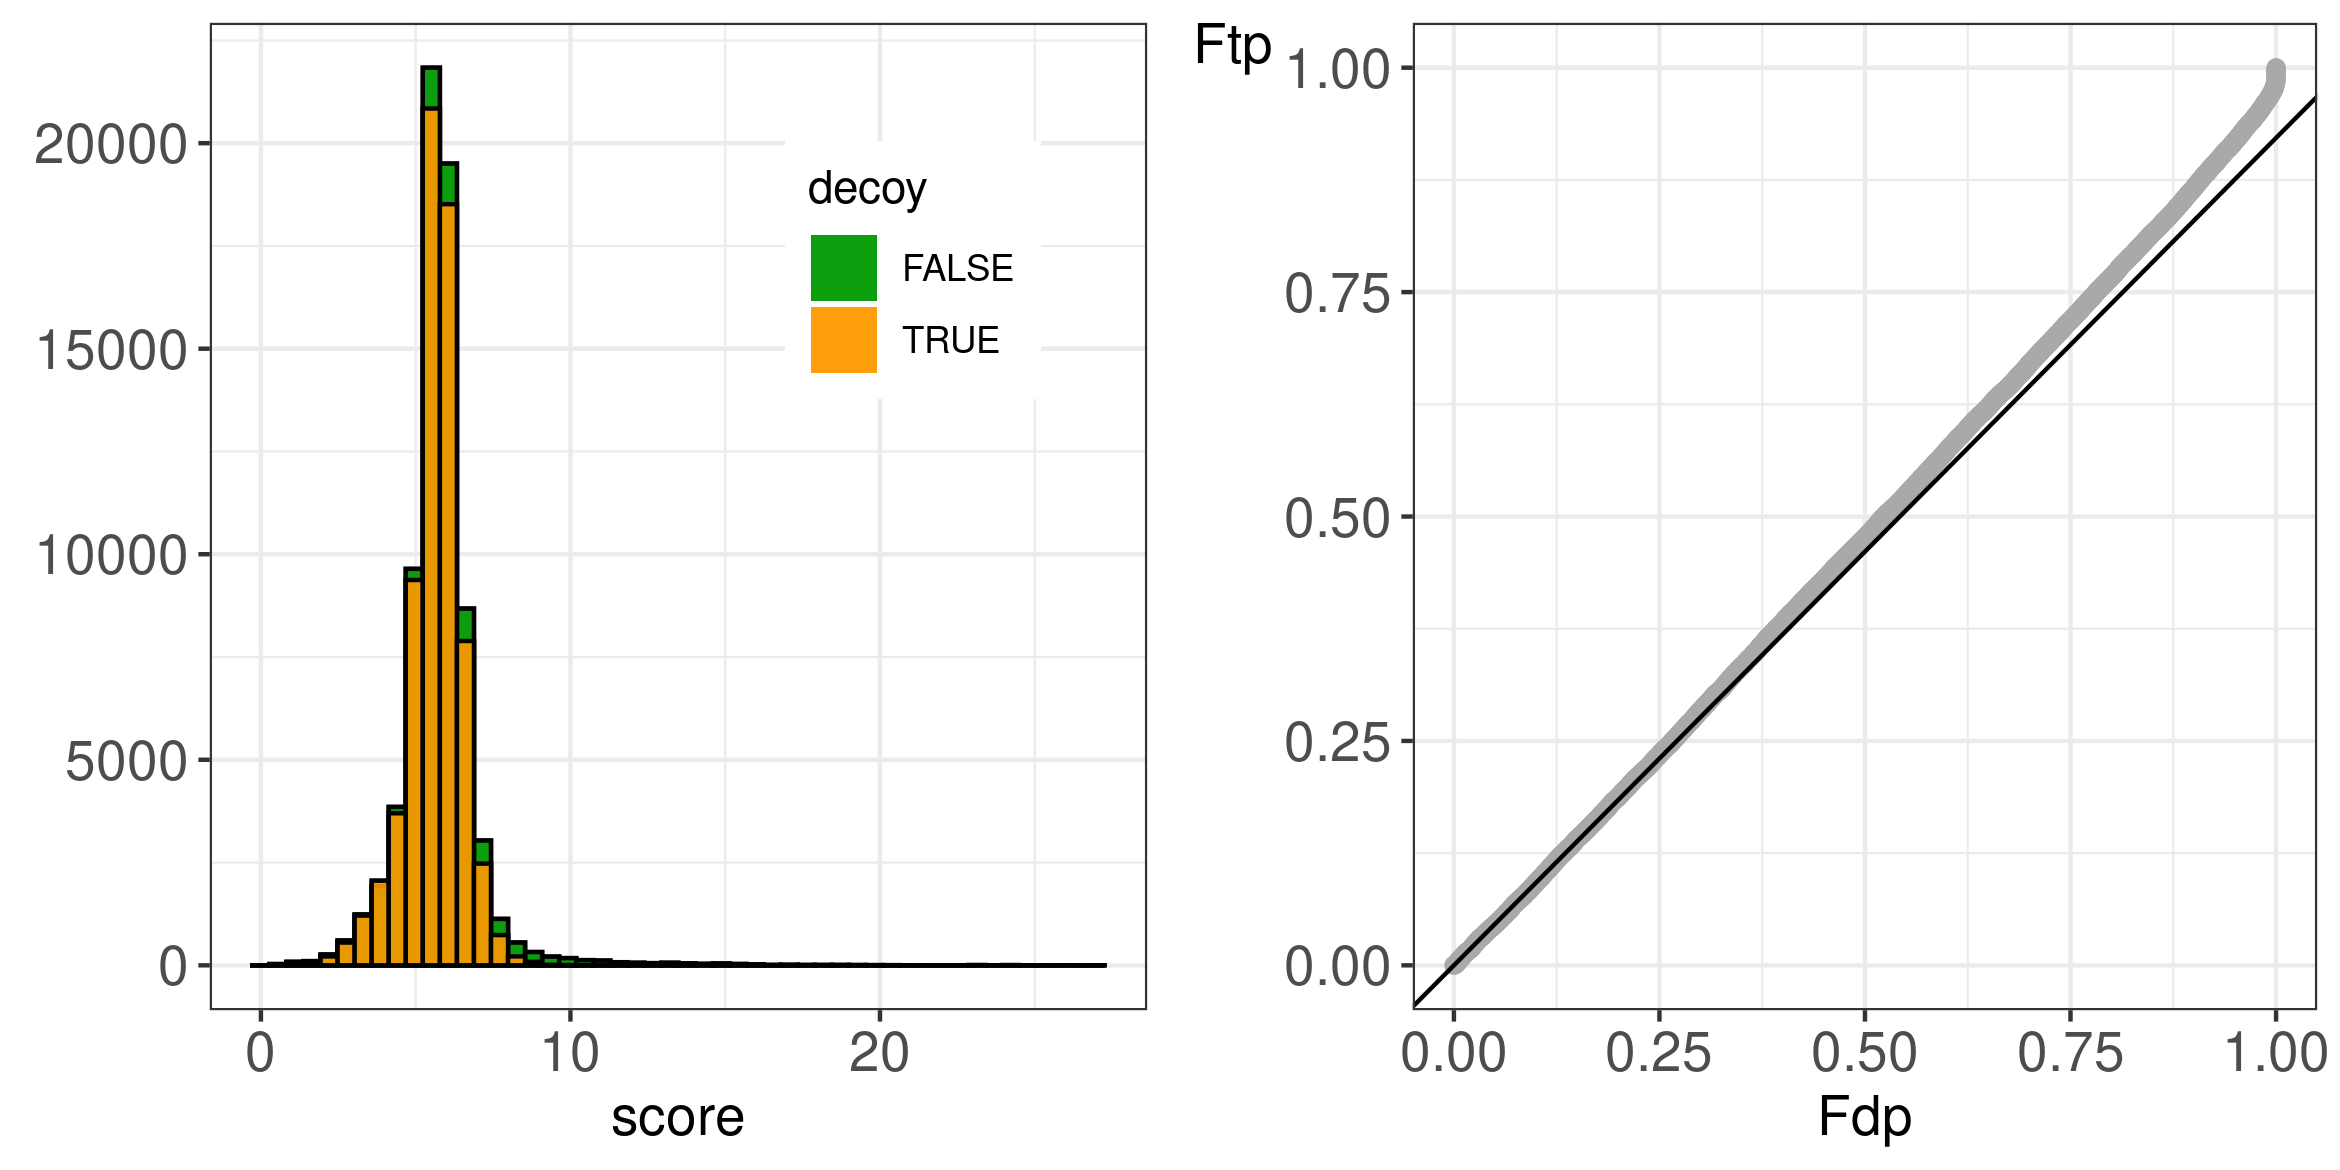
\includegraphics[width=0.99\linewidth]{./figs/figHumanMsgfPlusR2} \caption{Histogram and PP-plot for rank 2 target and decoy PSM scores of a concatenated search on a H. sapiens run against a database of H. Sapiens sequences from UniProt using MS-GF+.}\label{fig:sFig4}
\end{figure}

  \bibliography{biblio.bib}

\end{document}
